\noindent En este paso se procedió a realizar la calibración completa de los datos una vez realizada la calibración del primer día en el paso anterior. Para este caso, como parámetros iniciales $X_0$ para calibrar el día $t$, se utilizaron los parámetros óptimos obtenidos en el día anterior $(t-1)$.\\\\
El modelo fue calibrado obteniendo un conjunto de parámetros para cada de las fechas de los datos de mercado. A continuación se muestra como varía cada uno de los parámetros a través del tiempo:

\begin{figure}[H]
    \begin{center}
    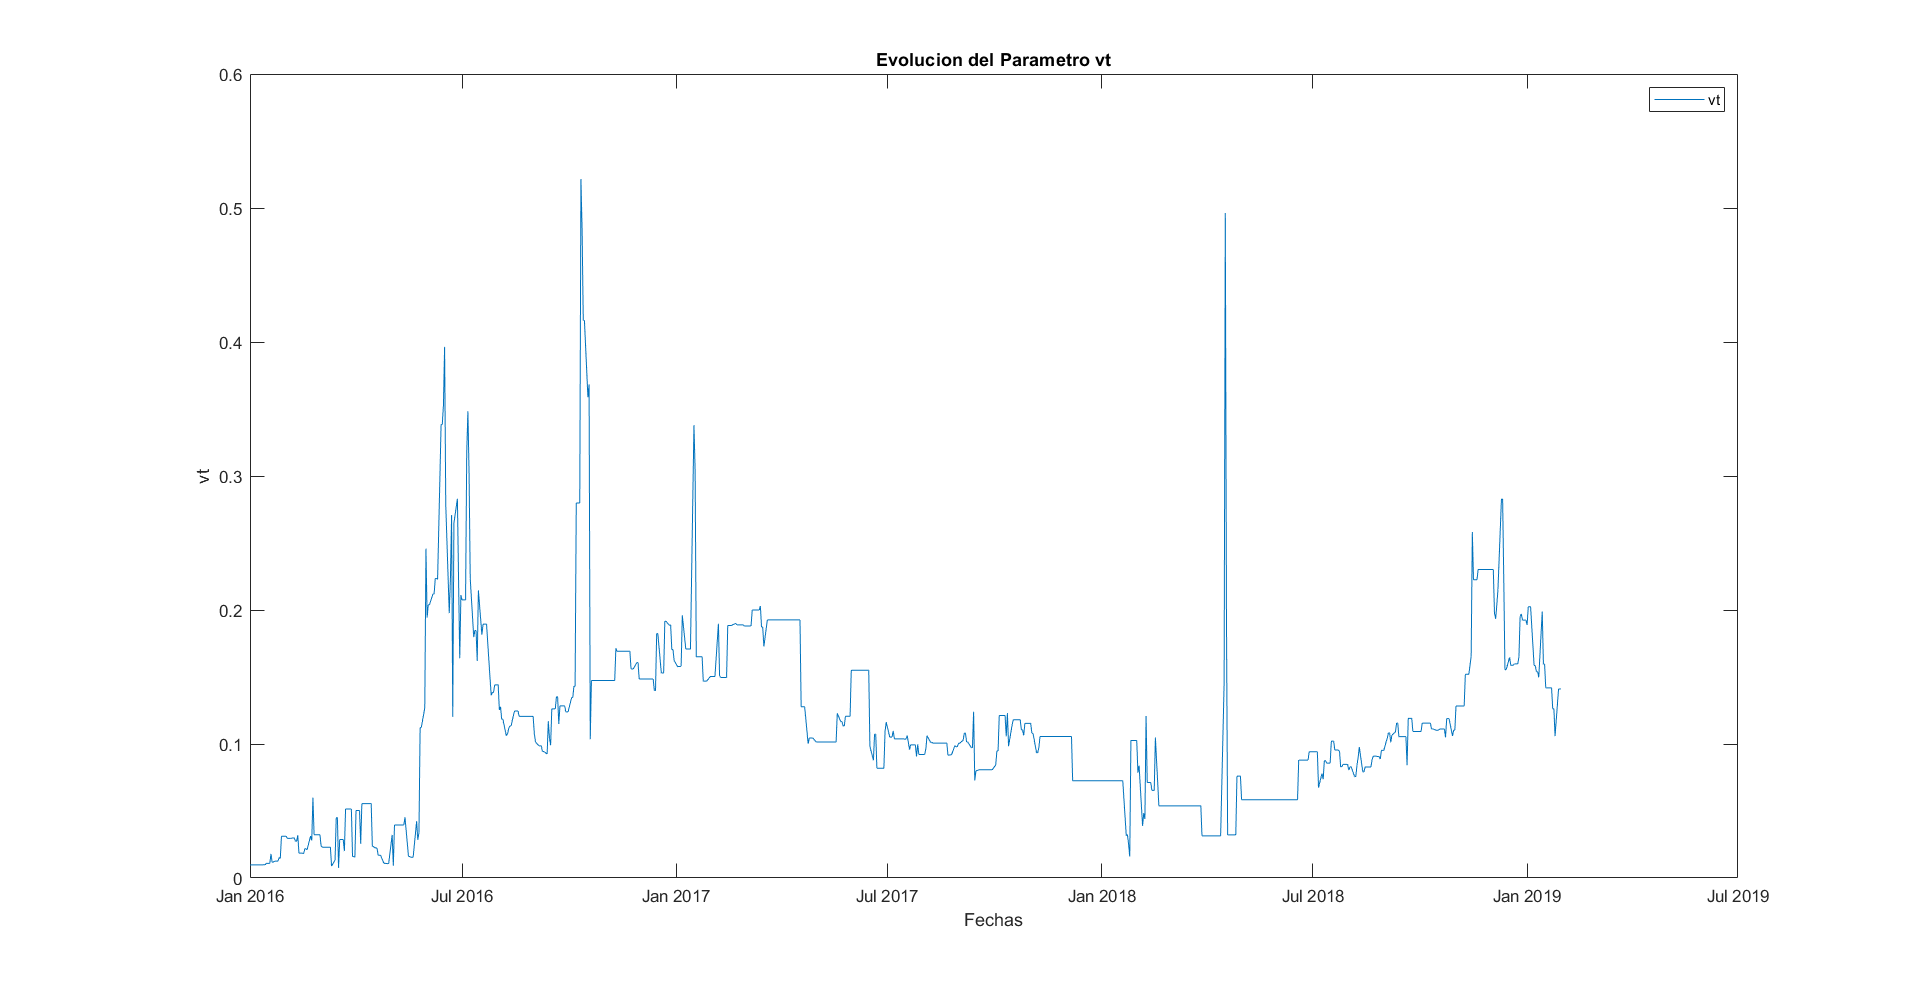
\includegraphics[width = 14cm]{figures/Evoluciondevt.png}
    \caption{$\nu_t$ en el tiempo}
    \label{nut} %El label permite citar el gráfico, pero es para más adelante
    \end{center}
\end{figure}
\begin{figure}[H]
    \begin{center}
    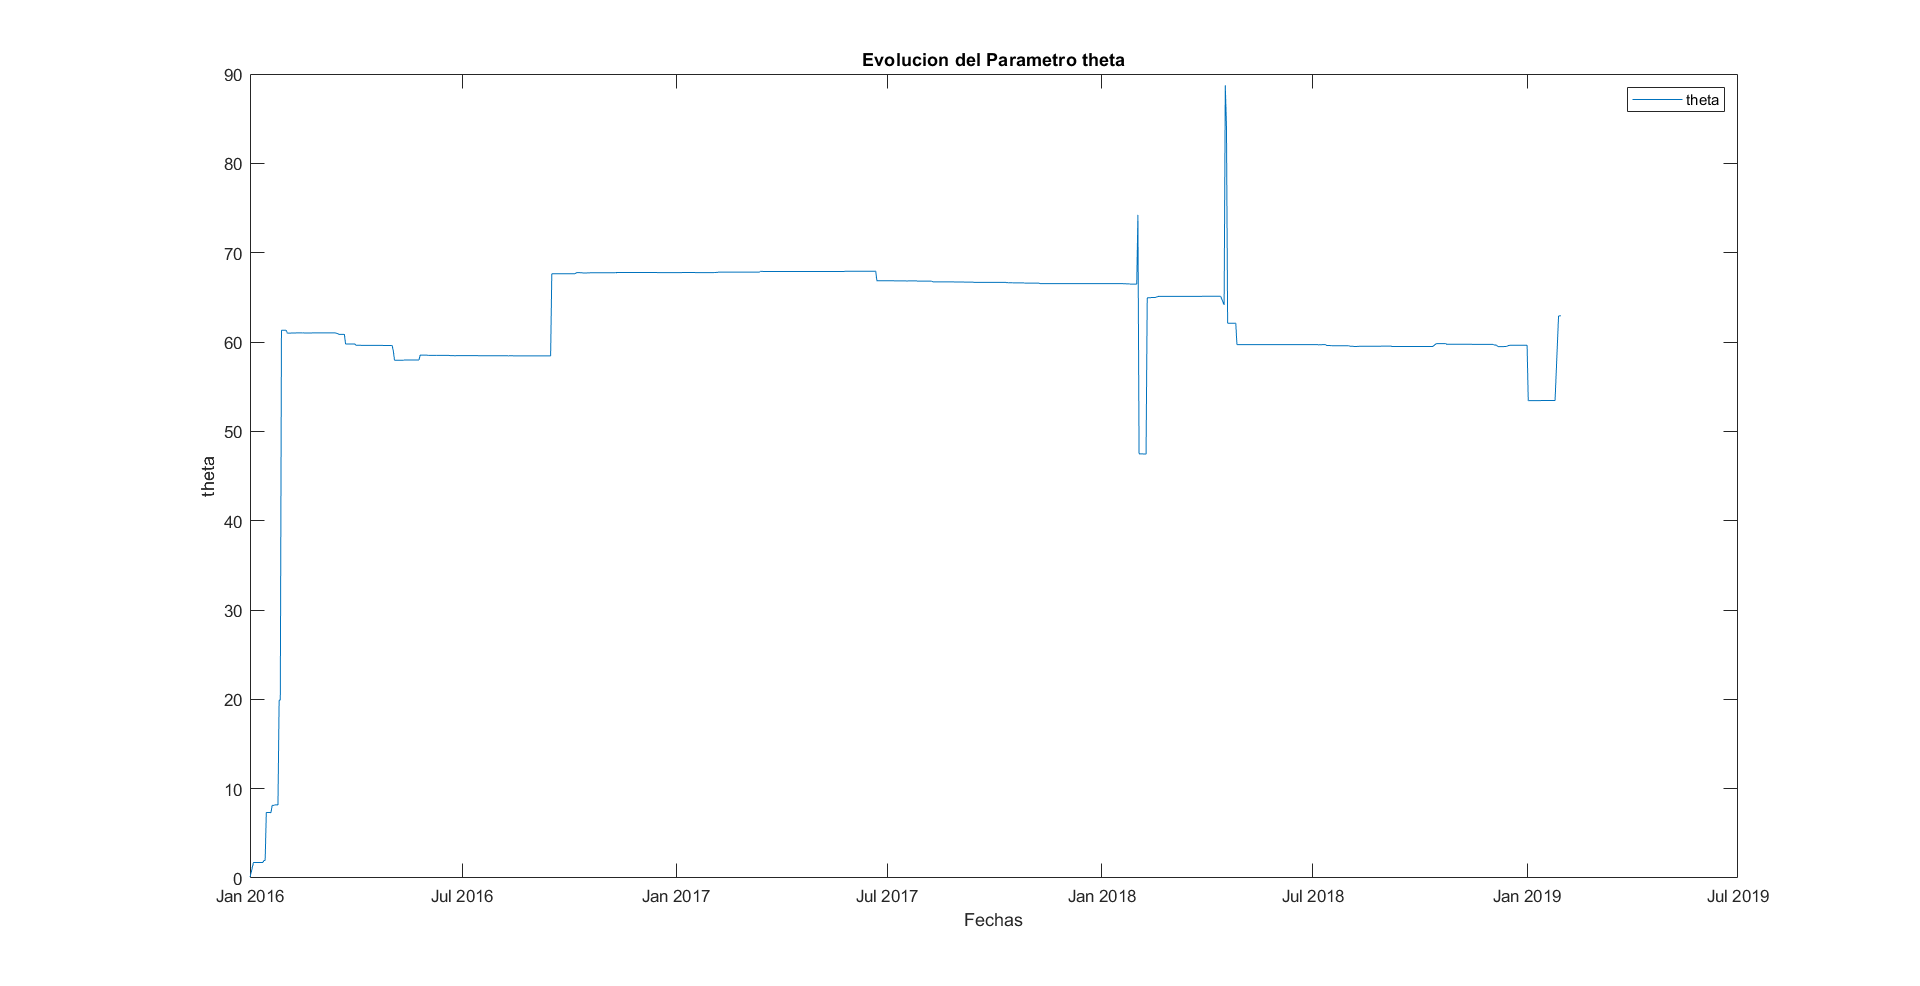
\includegraphics[width = 14cm]{figures/Evoluciondetheta.png}
    \caption{$\Theta$ en el tiempo}
    \label{theta} %El label permite citar el gráfico, pero es para más adelante
    \end{center}
\end{figure}
\begin{figure}[H]
    \begin{center}
    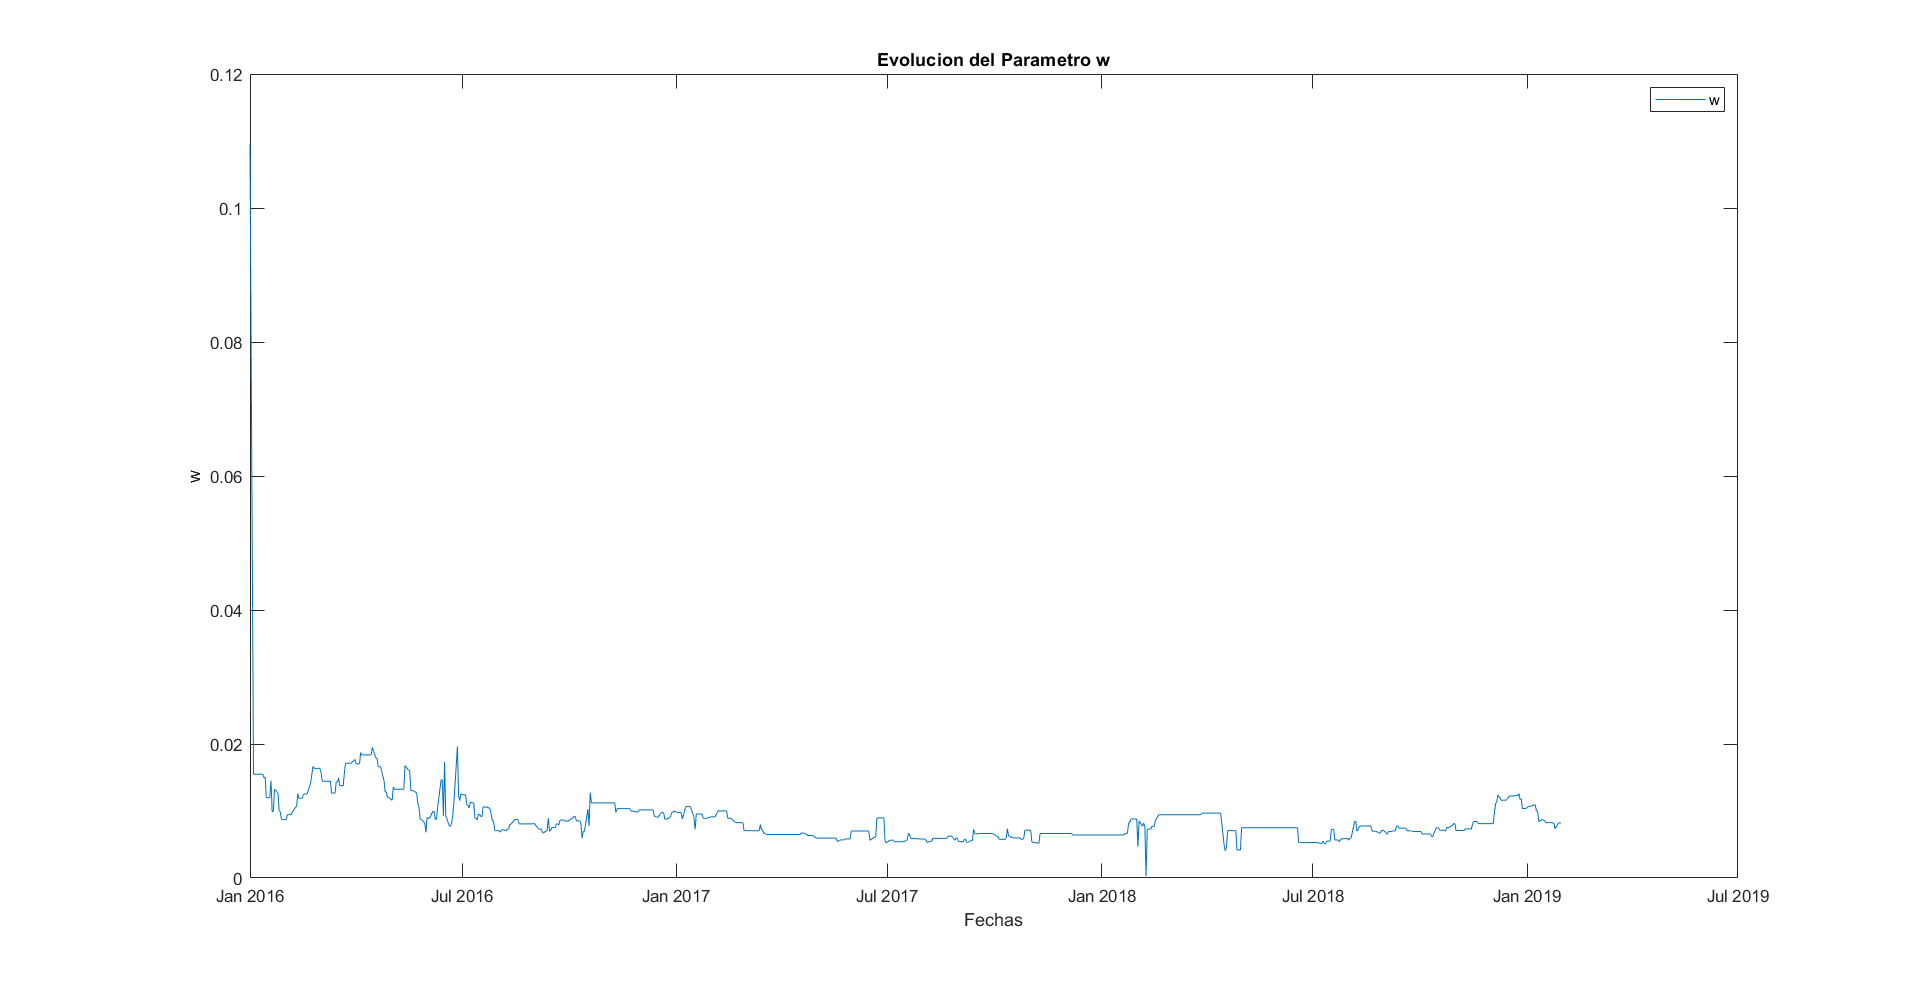
\includegraphics[width = 14cm]{figures/Evoluciondew.png}
    \caption{$\omega$ en el tiempo}
    \label{omega} %El label permite citar el gráfico, pero es para más adelante
    \end{center}
\end{figure}
\begin{figure}[H]
    \begin{center}
    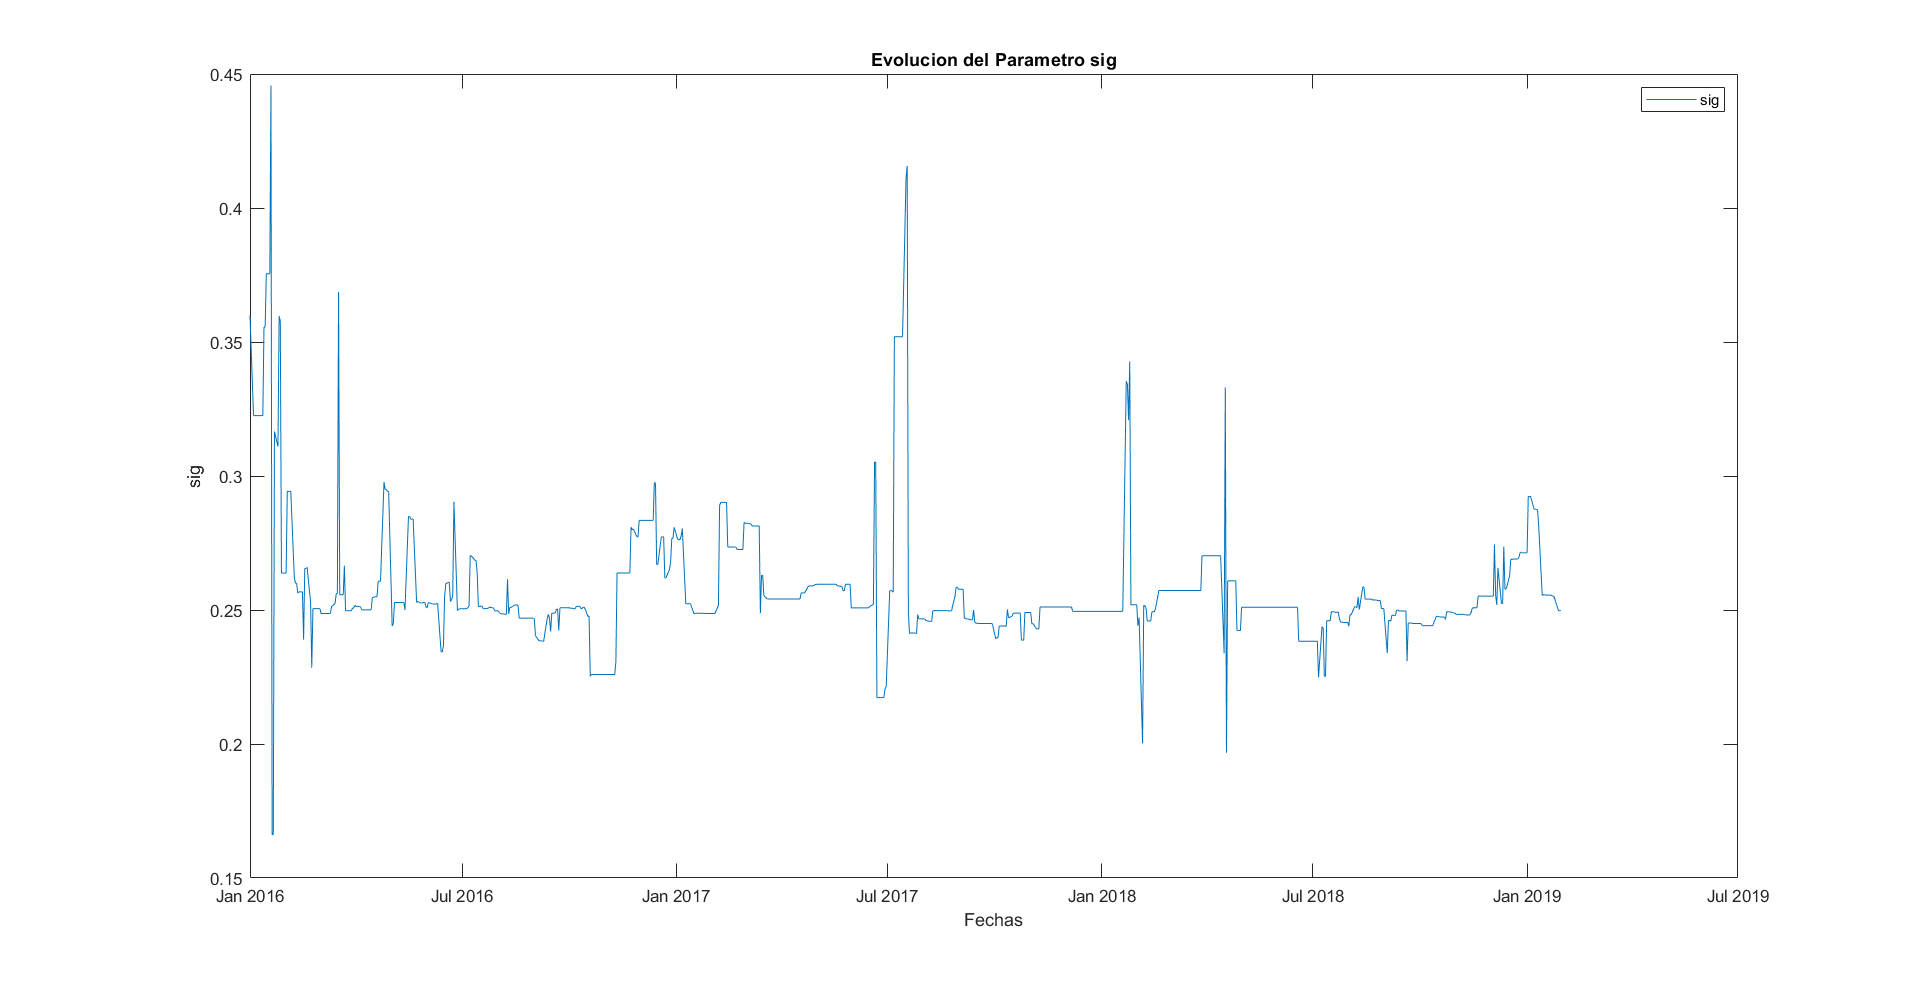
\includegraphics[width = 14cm]{figures/Evoluciondesig.png}
    \caption{$\xi$ en el tiempo}
    \label{xi} %El label permite citar el gráfico, pero es para más adelante
    \end{center}
\end{figure}
\begin{figure}[H]
    \begin{center}
    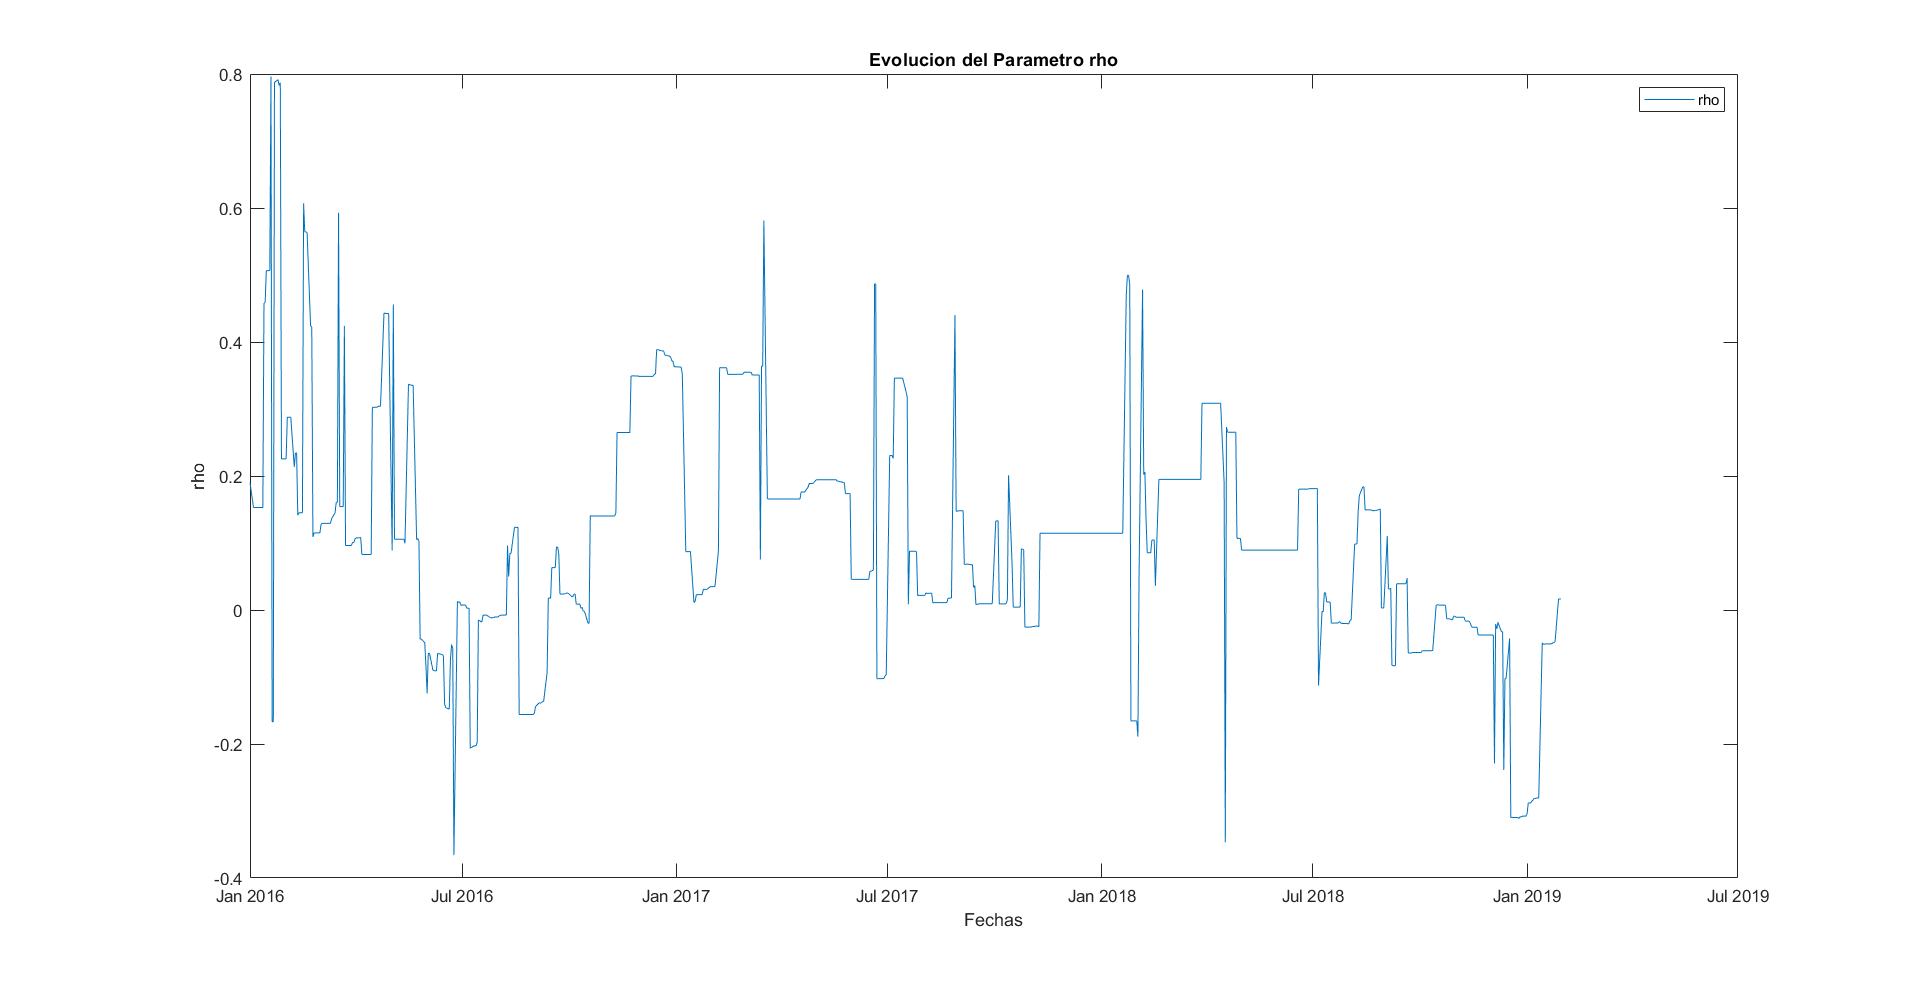
\includegraphics[width = 14cm]{figures/Evolucionderho.png}
    \caption{$\rho$ en el tiempo}
    \label{rho} %El label permite citar el gráfico, pero es para más adelante
    \end{center}
\end{figure}

\noindent Por otra parte, se presentan las curvas \textit{Smile} para los diferentes tenores, tanto como para la volatilidad del modelo como la del mercado. A continuación, se muestran las diferentes curvas Smile: 
\begin{figure}[H]
    \begin{center}
    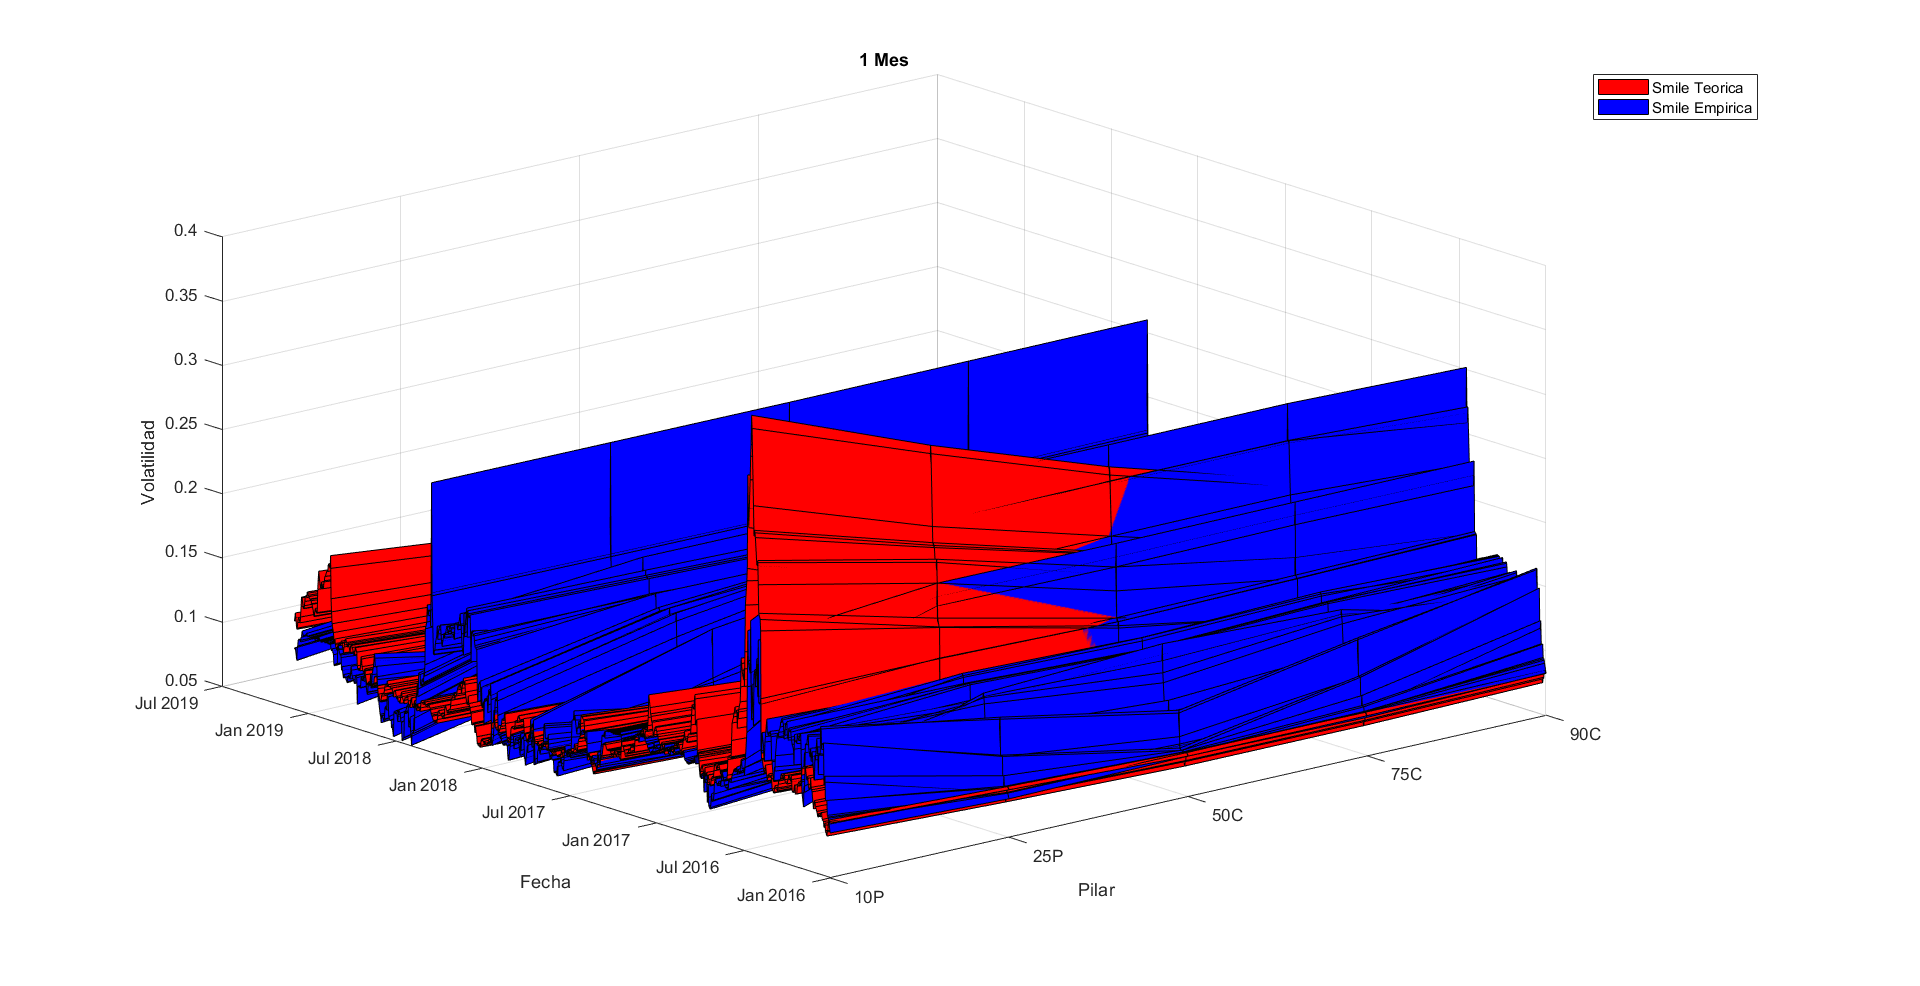
\includegraphics[width = 14cm]{figures/Smile3d1Mes.png}
    \caption{Curva Smile para 1 Mes}
    \label{Smile1} %El label permite citar el gráfico, pero es para más adelante
    \end{center}
\end{figure}
\begin{figure}[H]
    \begin{center}
    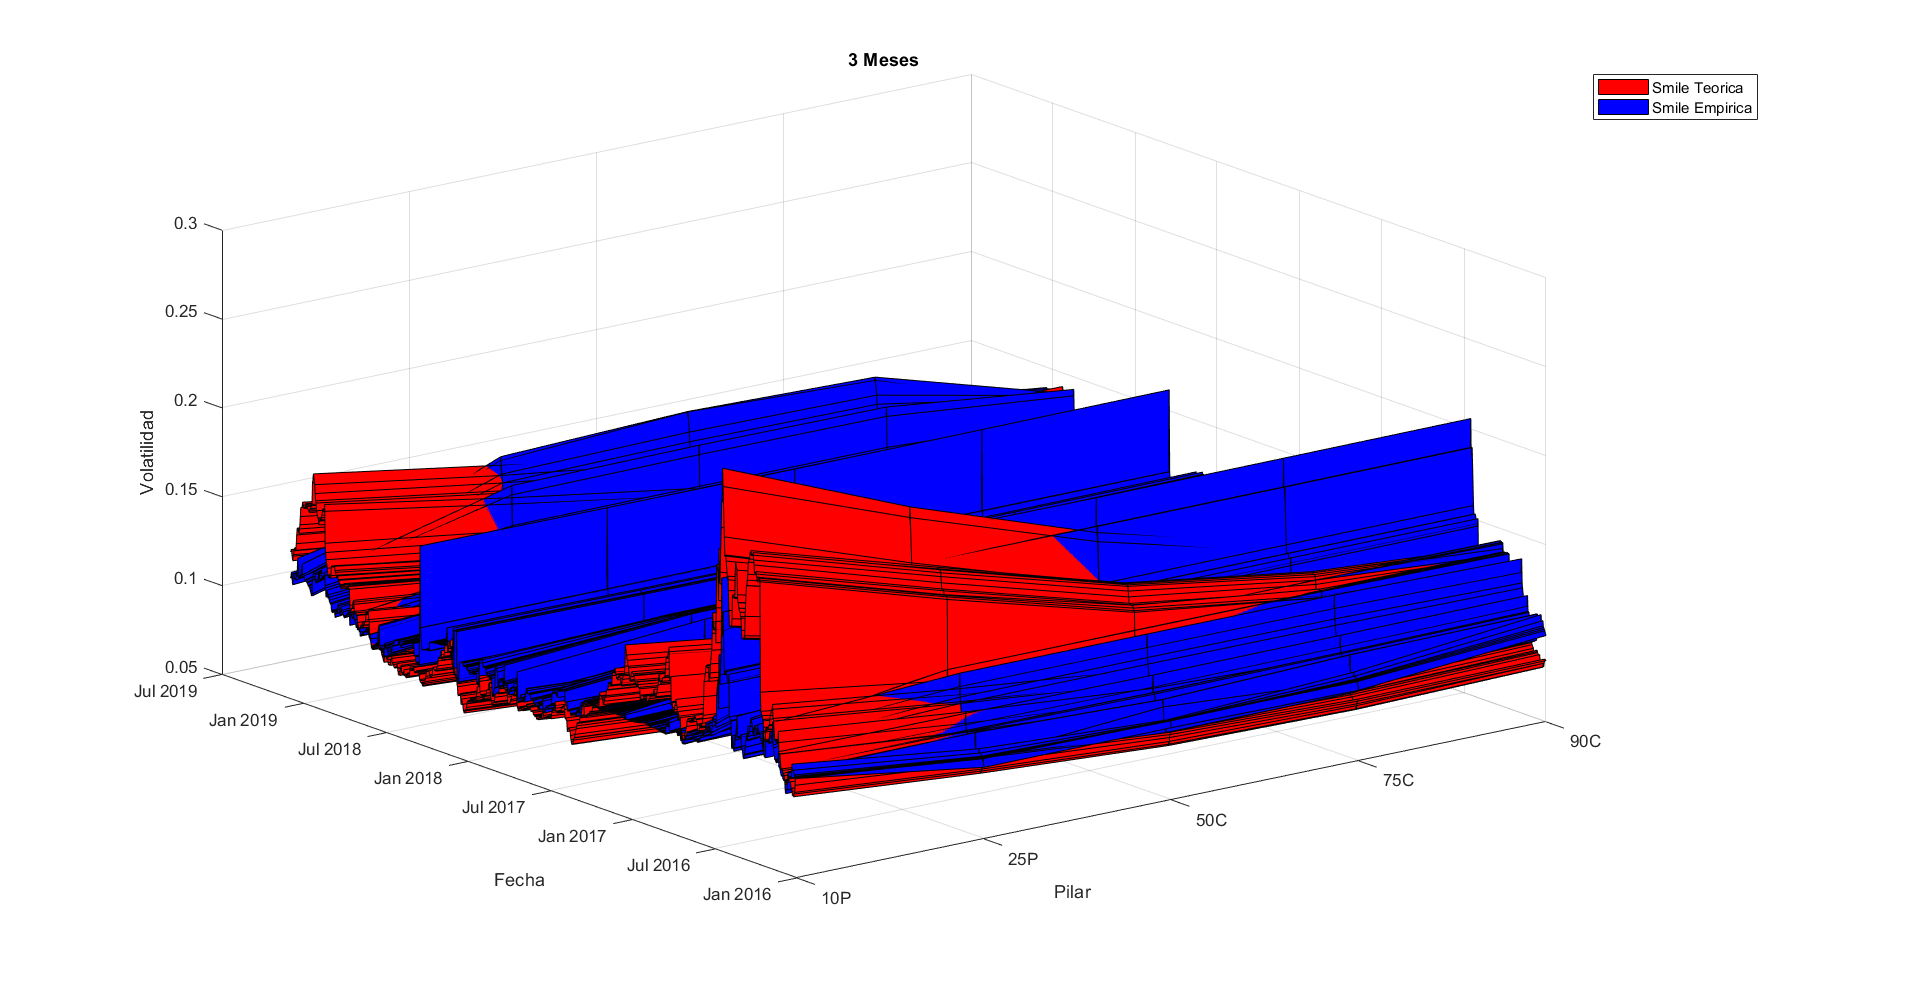
\includegraphics[width = 14cm]{figures/Smile3d3Meses.png}
    \caption{Curva Smile para 3 Meses}
    \label{Smile2} %El label permite citar el gráfico, pero es para más adelante
    \end{center}
\end{figure}
\begin{figure}[H]
    \begin{center}
    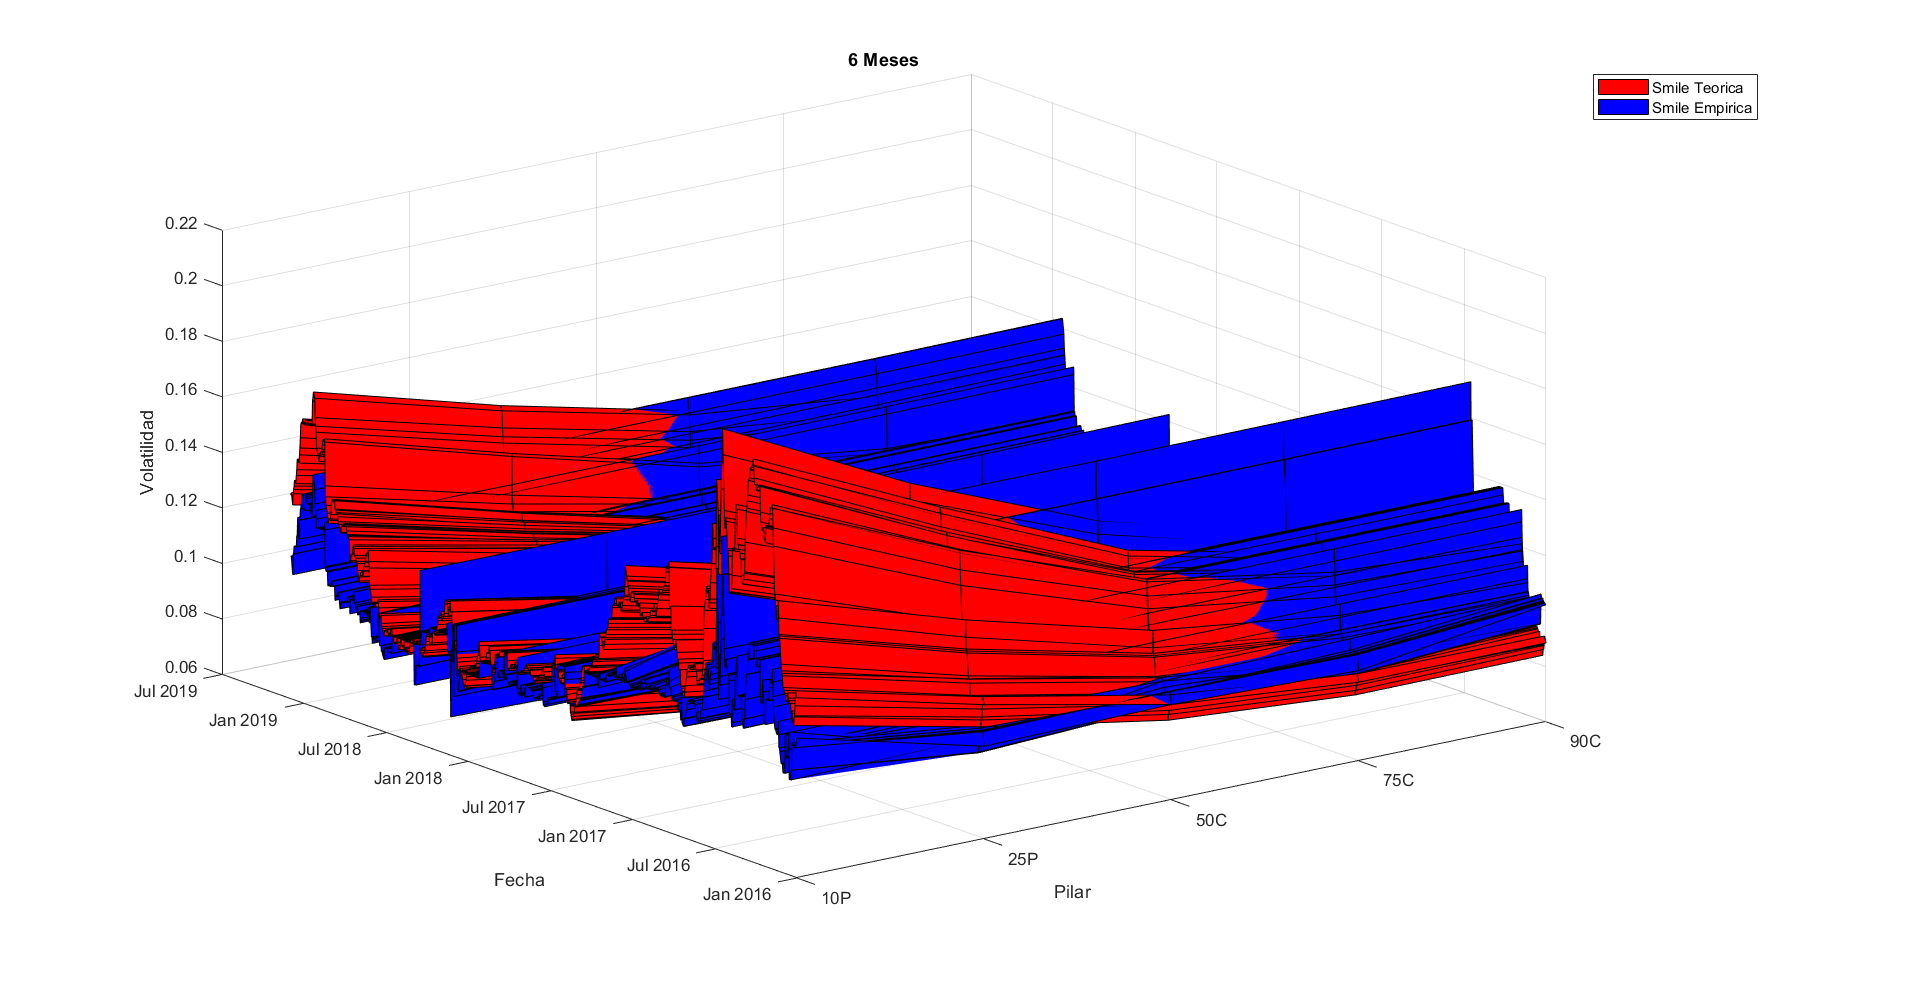
\includegraphics[width = 14cm]{figures/Smile3d6Meses.png}
    \caption{Curva Smile para 6 Meses}
    \label{smile3} %El label permite citar el gráfico, pero es para más adelante
    \end{center}
\end{figure}
\begin{figure}[H]
    \begin{center}
    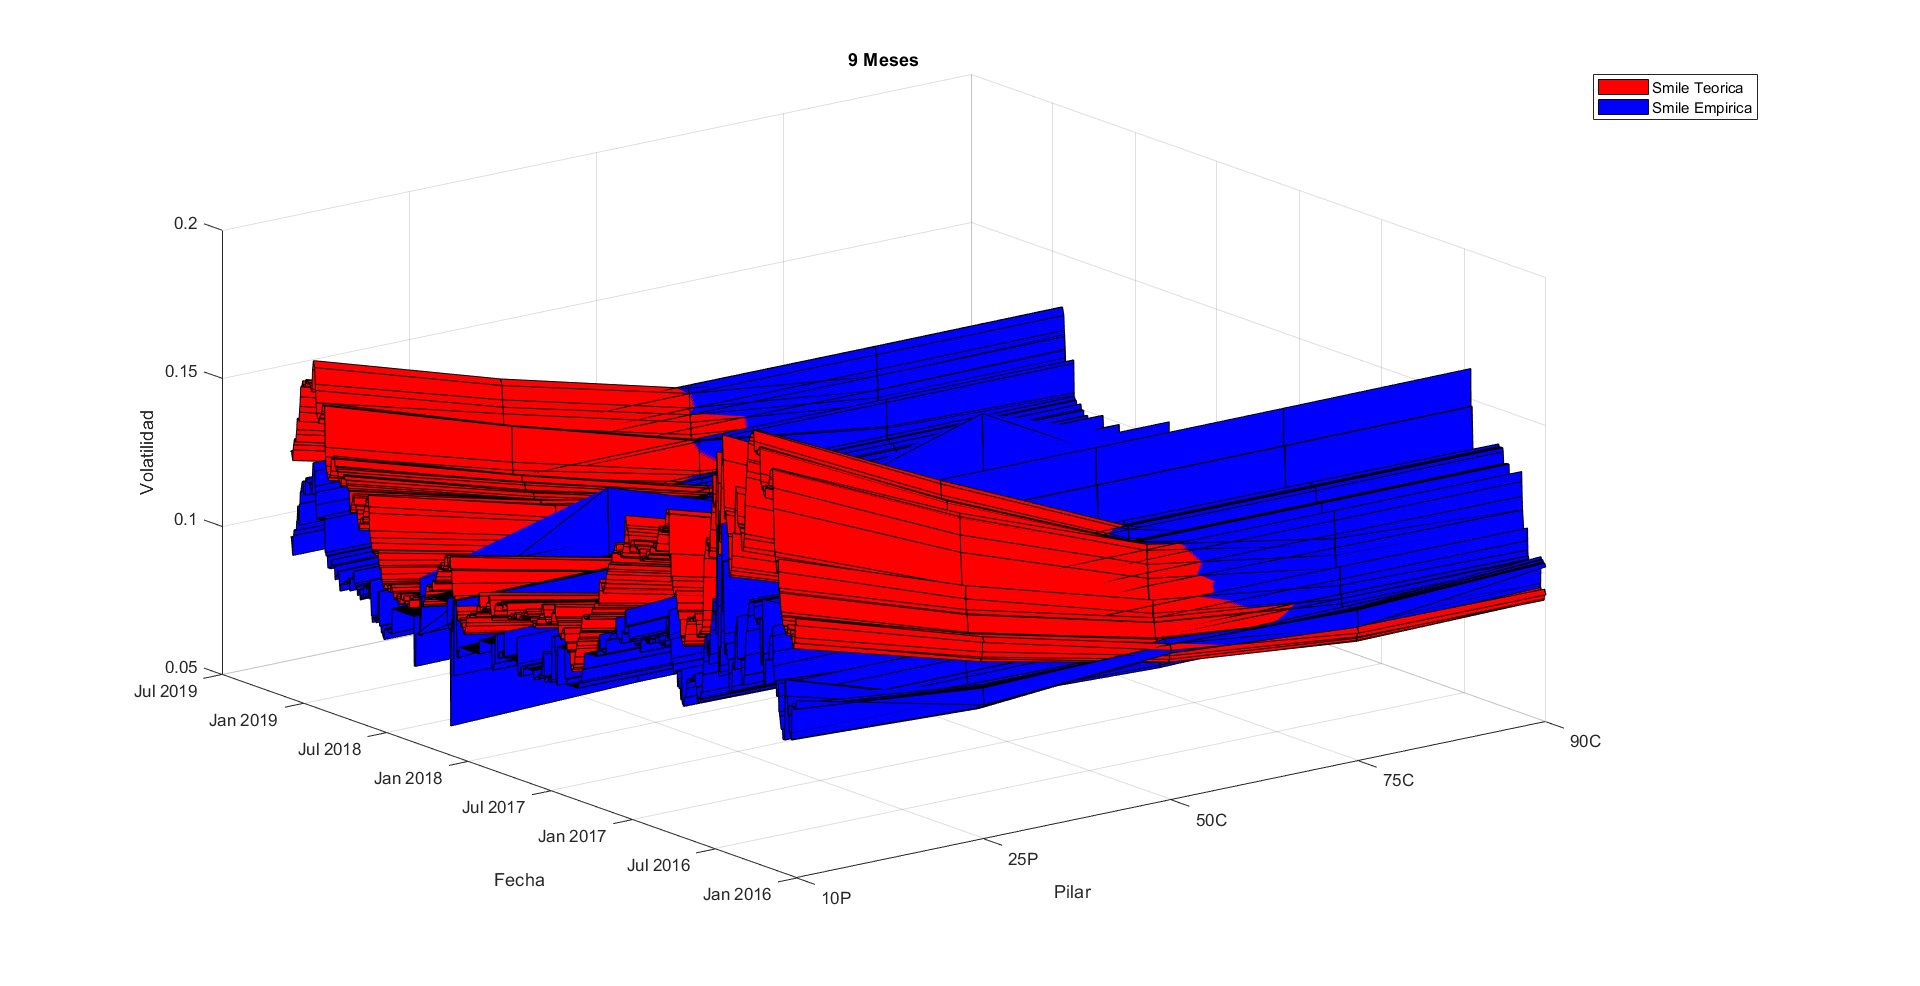
\includegraphics[width = 14cm]{figures/Smile3d9Meses.png}
    \caption{Curva Smile para 9 Meses}
    \label{smile4} %El label permite citar el gráfico, pero es para más adelante
    \end{center}
\end{figure}
\begin{figure}[H]
    \begin{center}
    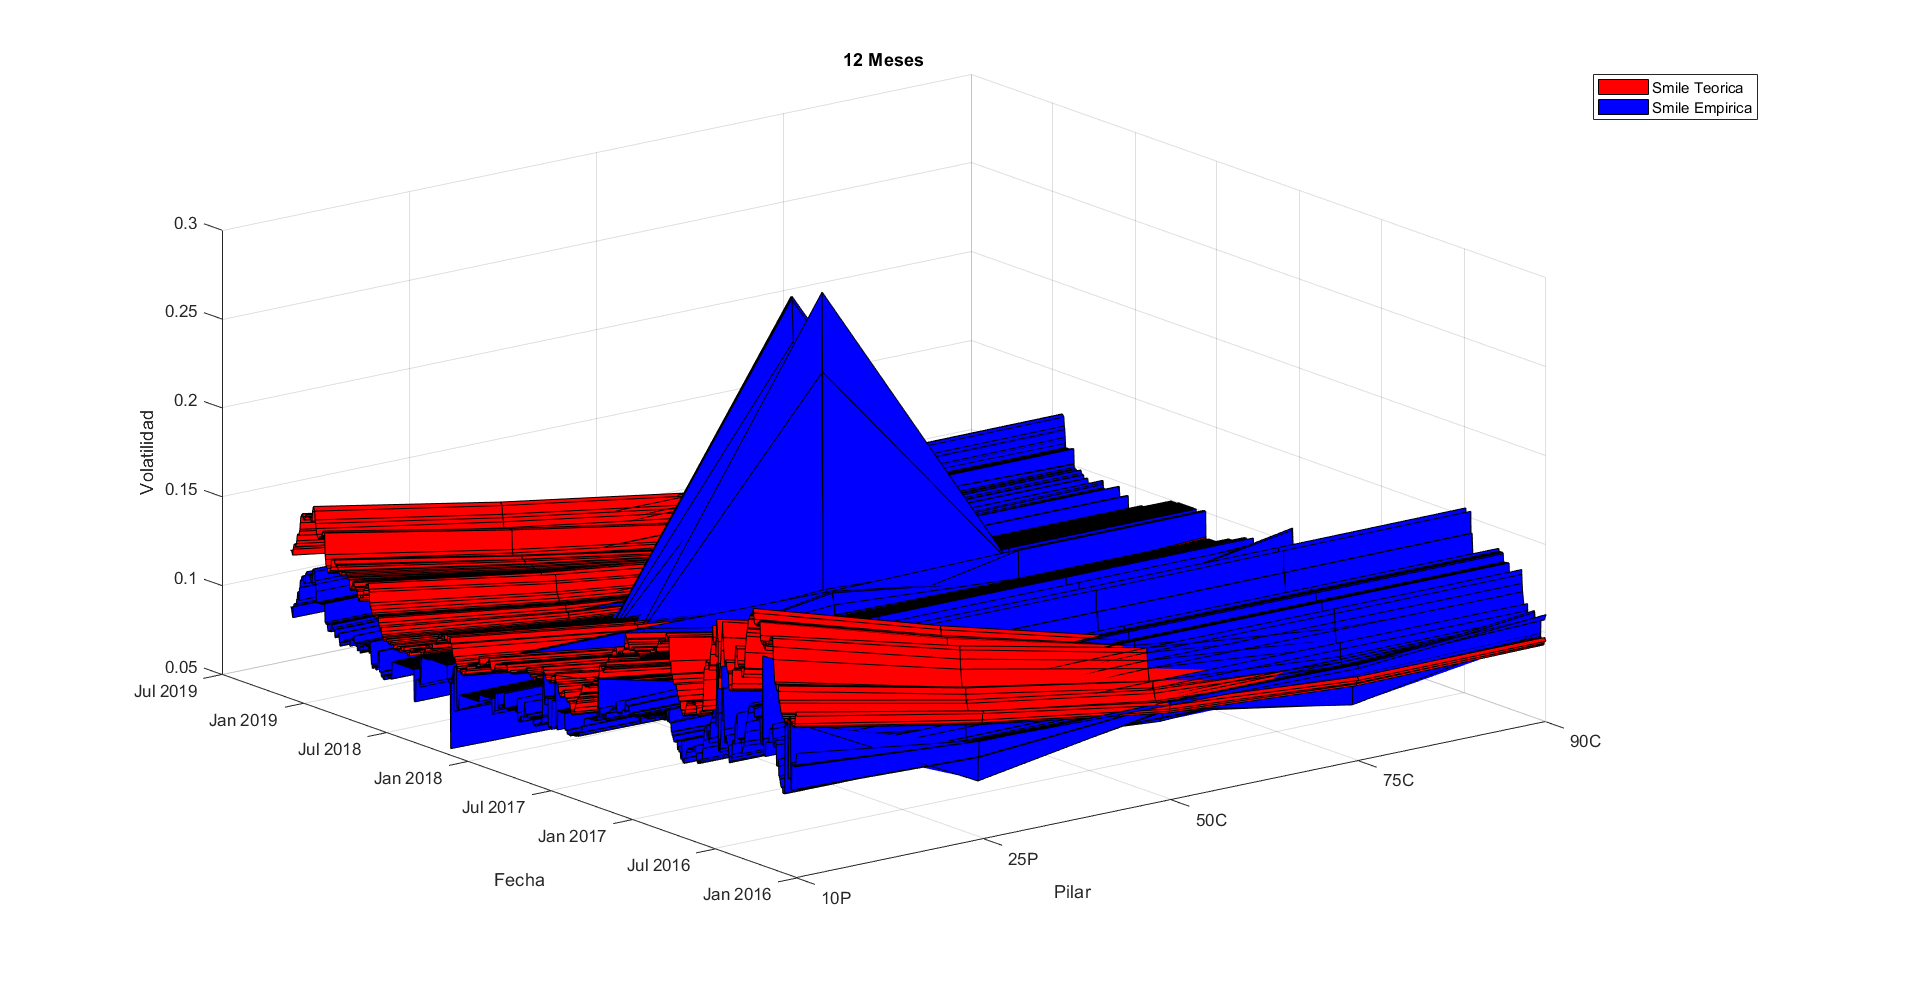
\includegraphics[width = 14cm]{figures/Smile3d12Meses.png}
    \caption{Curva Smile para 12 Meses}
    \label{smile5} %El label permite citar el gráfico, pero es para más adelante
    \end{center}
\end{figure}

\noindent Por otra parte, también se calcularon los errores obtenidos para todo el conjunto de datos, en el cual existe un error promedio de 0.015251, correspondiente a un error promedio porcentual del 14.7394\%.\\\\
\noindent Finalmente, se graficó como se comporta el error promedio $\epsilon$ para cada uno de los 804 días, entregando la siguiente gráfica:
\begin{figure}[H]
    \begin{center}
    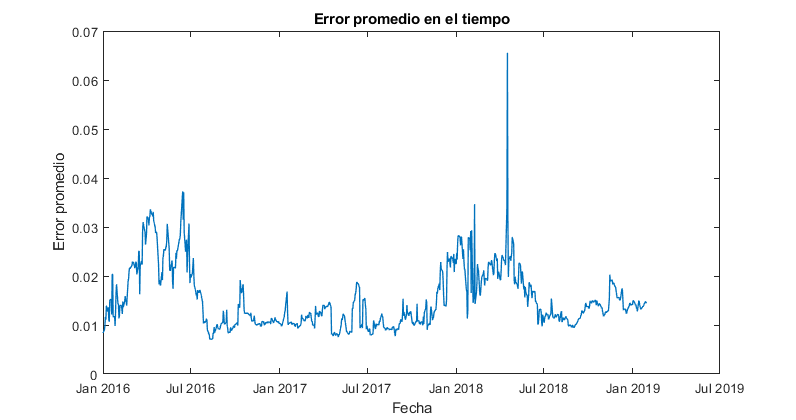
\includegraphics[width = 14cm]{figures/ErrorPromedioVsTiempo.png}
    \caption{Error promedio en el tiempo}
    \label{errorpromedio} %El label permite citar el gráfico, pero es para más adelante
    \end{center}
\end{figure}

\noindent Como se puede observar, existe un periodo cercano a Julio del 2018 donde $\epsilon$ alcanza un máximo local. Dicho error se lo podemos atribuir a como cambia de forma drástica el \textit{Spot Price} en este periodo, lo cual se puede observar en la siguiente figura:
\begin{figure}[H]
    \begin{center}
    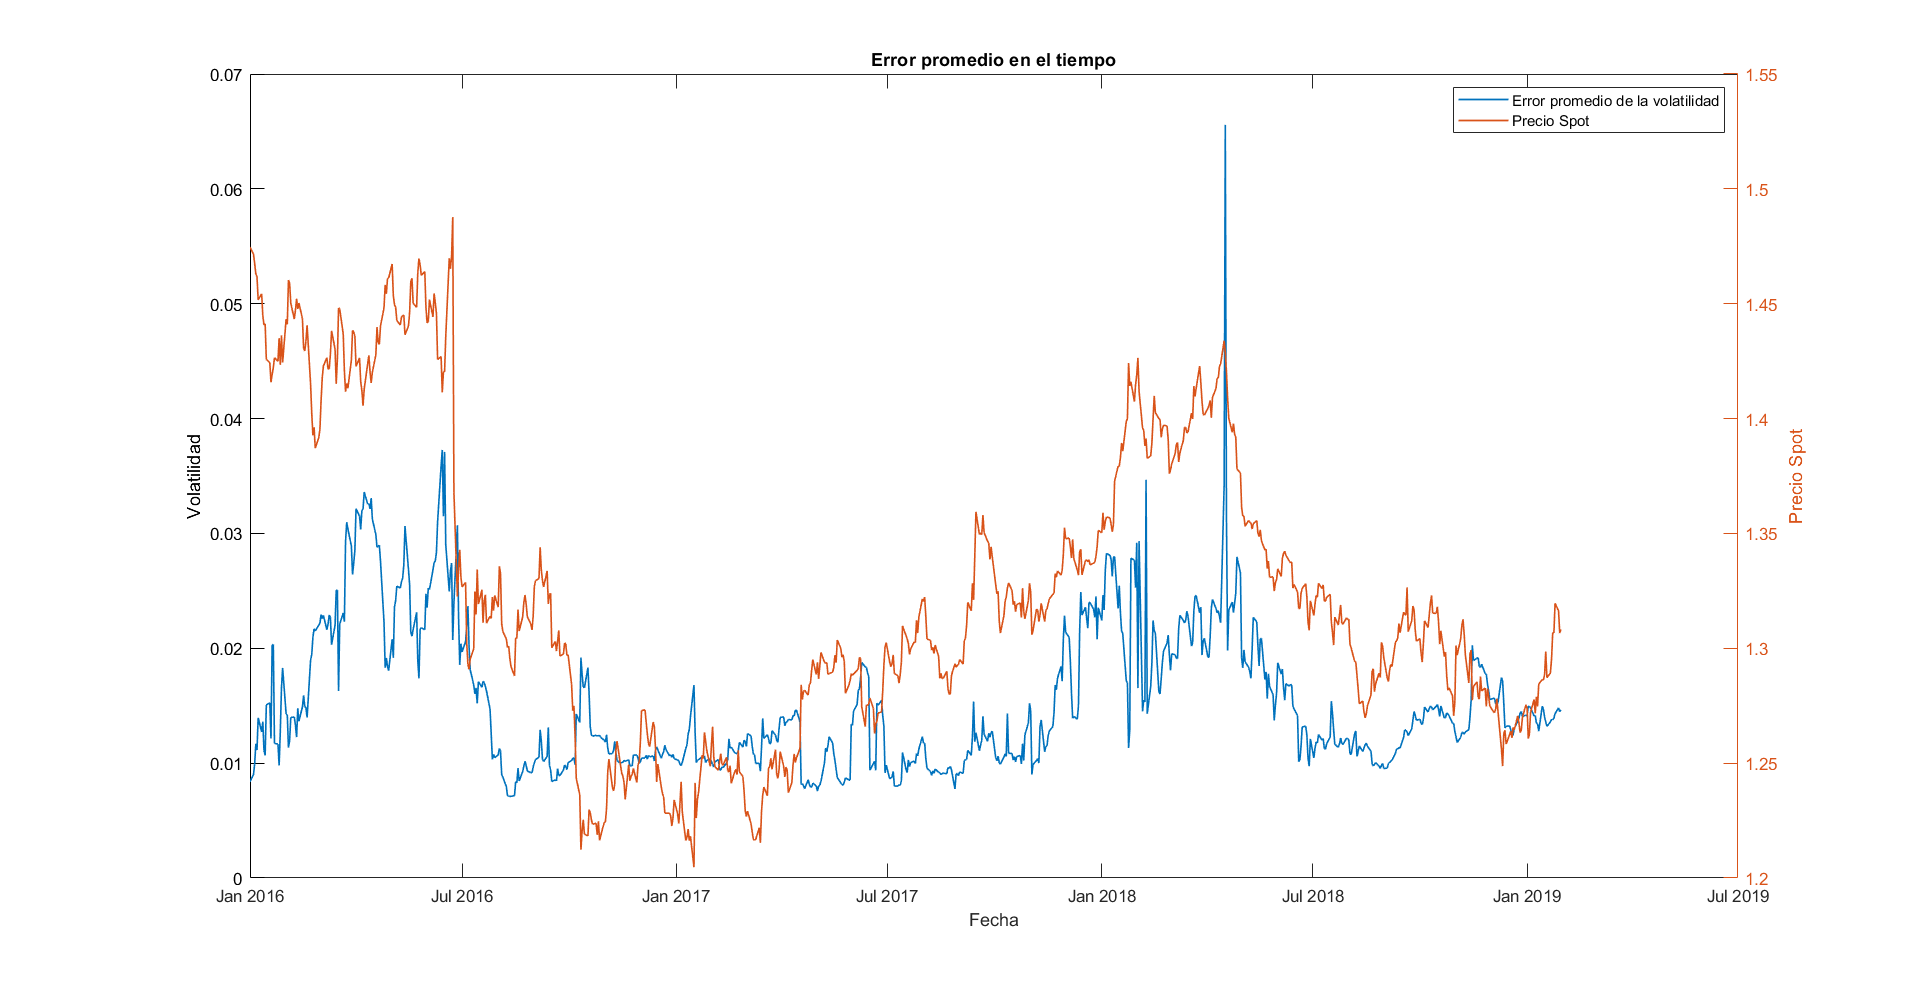
\includegraphics[width = 14cm]{figures/Errorpromediovolatilidad.png}
    \caption{Error promedio volatilidad y Precio Spot}
    \label{error4} %El label permite citar el gráfico, pero es para más adelante
    \end{center}
\end{figure}
\newpage


